\documentclass{article}
\usepackage{blindtext}
\usepackage[utf8]{inputenc}
\usepackage{graphicx}

\author{Nistor Marian-Sergiu, 3B6}
\title{%
  	\textbf{Securitatea Informatiei} \\
  	\textbf{\large{Tema 1}} \\
}

\begin{document}

\maketitle



\section{Introducere}
Aplicatia implica o retea, bazata pe arhitectura TCP Server-Client, in care comunicarea se realizeaza criptat.


\section{Premise}
Atat Serverul, cat si Clientul, pot fi executate pe orice mediu Linux, inclusiv WSL(Windows Subsystem for Linux). \\
Este necesar ca pe sistemul respectiv sa fie instalat libopenssl, spre a avea acces la primitivele de incriptie.


\section{Compilare}
Serverul si Clientul au, fiecare, un "Makefile", care poate fi executat la linia de comanda, astfel:
\begin{verbatim}
./Makefile
\end{verbatim}
In urma executiei Makefile-ului, sunt generate executabilele, plasate in folderul "bin".


\section{Resurse}
Atat in cazul Serverului, cat si al Clientului, cheia si vectorul de initializare folosite pentru comunicarea initiala cu Serverul, se regasesc in folderul "resources", in fisierele "key.pem" si, respectiv, "iv.pem".


\section{Mod de Utilizare}
In primul rand, o instanta a Serverului trebuie sa fie pornita. Executabilul de Server se regaseste in folderul "bin". Nu este necesara pasarea vreunui argument la linia de comanda. \\
Executabilul de Client se regaseste in folderul "bin". Trebuie pasat un argument la linia de comanda, specificand modul de operare folosit("ecb"/"ECB" ori "cfb"/"CFB"). Daca argumentul este invalid, Clientul va folosi CFB. \\
Serverul va astepta conexiuni. Dupa conectarea unui Client, toti ceilalti Clienti sunt notificati. Apoi, se asteapta un mesaj din partea noului Client, in cadrul caruia mentioneaza daca doreste sa foloseasca modul de operare ECB, ori CFB, pentru incriptia AES. Dupa receptionarea mesajului, se creaza o cheie noua si un vector de initializare(random, folosind primita RAND\_bytes() din headerul "openssl/rand.h" a bibliotecii openssl. Acestea sunt trimise, pe rand, catre client. Din acel punct, Clientul respectiv este plasat in pool-ul de Clienti conectati. \\
Cand un Client trimite un mesaj, acesta este decriptat de catre server si recriptat, conform cheilor si vectorilor de initializare asociate fiecarui altui Client, ca apoi criptotextele sa fie trimise catre ceilalti Clienti. \\
In momentul in care un Client se deconecteaza, Serverul detecteaza acest eveniment si notifica toti ceilalti Clienti.


\section{Modalitati de Incriptie}
Dupa realizarea conexiunii Serverului cu un Client, mesajul in care Clientul specifica modalitatea de incriptie dorita este criptat folosind modul de operare CFB, avand la dispozitie cheia si vectorul de initializare din fisierele "key.pem" si "iv.pem". Raspunsul Serverului(continand o noua cheie si un nou vector de initializare, care urmeaza sa fie folosite in comunicarea cu Clientul) va fi, de asemenea, incriptionat folosind cheia si vectorul de initializare initial. \\
Fiecarui Client ii este asociata o cheie si un vector de initializare, care sunt generate random la momentul conectarii sale. Pana la terminarea conexiunii, Serverul va comunica cu acel Client folosind respectiva cheie si respectivul vector de initializare.


\section{Implementari Moduri de Operare}
Pentru a implementa modurile de operare ECB si CFB, s-au folosit primitivele "aes\_encrypt" si "aes\_decrypt" din headerul "openssl/aes.h" a bibliotecii openssl.

\subsection{ECB}
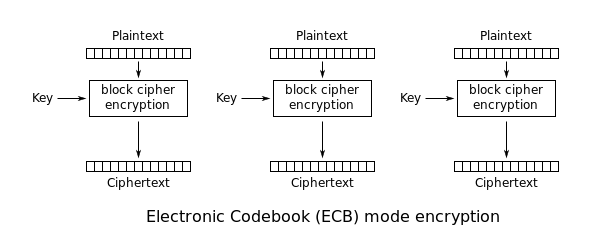
\includegraphics[width=\textwidth,height=\textheight,keepaspectratio]{ECB_Encryption.png} \\
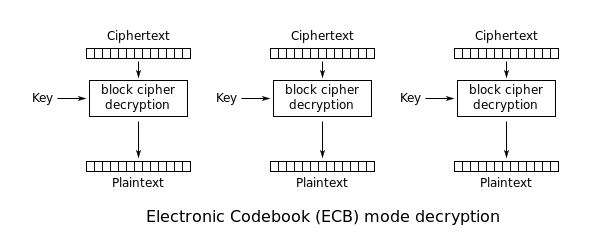
\includegraphics[width=\textwidth,height=\textheight,keepaspectratio]{ECB_Decryption.png} \\

\subsection{CFB}
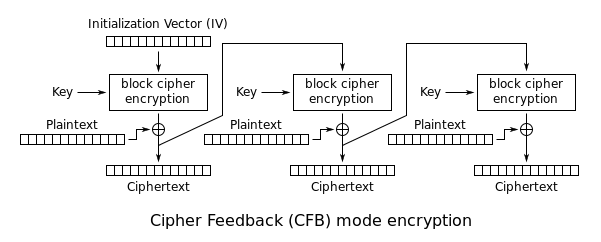
\includegraphics[width=\textwidth,height=\textheight,keepaspectratio]{CFB_Encryption.png} \\
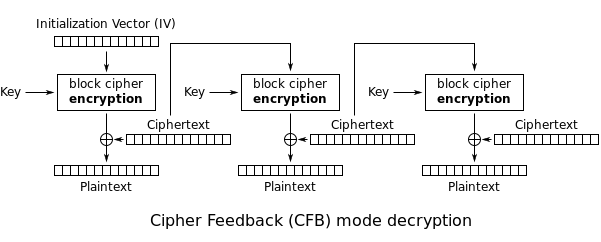
\includegraphics[width=\textwidth,height=\textheight,keepaspectratio]{CFB_Decryption.png} \\


\end{document}